\documentclass[11pt a4paper]{article}
\usepackage[greek,english]{babel}
\usepackage{amsmath,amssymb,amsthm}
\usepackage{mathrsfs,bm}
\usepackage{graphicx,epstopdf,caption}
\usepackage{float,subcaption,setspace,booktabs,multirow,supertabular,lscape,threeparttable}
\usepackage{float,colortbl}
\usepackage{placeins}
\usepackage{indentfirst}
\usepackage{enumitem}
\setlength{\parindent}{2em} %% noindent for the entire file % or add indent {2em}
\usepackage{geometry}
\geometry{left=0.8in,right=0.8in,top=1in,bottom=1in}
\usepackage[noblocks]{authblk}
\usepackage{lipsum}%% a garbage package you don't need except to create examples.
\usepackage{fancyhdr}
\pagestyle{fancy}
\renewcommand{\headrulewidth}{0.4pt}
\usepackage[svgnames]{xcolor}
\usepackage{listings}
\usepackage{verbatim}
\lstset{language=R,
	basicstyle=\small\ttfamily,
	stringstyle=\color{DarkGreen},
	otherkeywords={0,1,2,3,4,5,6,7,8,9},
	morekeywords={TRUE,FALSE},
	deletekeywords={data,frame,length,as,character},
	keywordstyle=\color{blue},
	commentstyle=\color{DarkGreen},
}
\usepackage{blindtext}
\usepackage{scrextend}
\addtokomafont{labelinglabel}{\bfseries}
\usepackage{xcolor}
\usepackage{csvsimple}

% set the section margin and font size
\usepackage[compact, small]{titlesec}

\graphicspath{{Figures/}}  % set the path of figures
\rhead{November}  % set your name here
\lhead{Applied Exam Q2} % set the document name here

\begin{document}
	
	\title{\vspace{-1in}Applied Exam Problem 2}
	\author{November}  %% set your name on the main page
	\date{\vspace{-5ex}}  % suppress the output of date
	\maketitle
	
	\section{Introduction}
	This report is a summary of my work for Problem 2. In Section \ref{sec: eda}, data exploration and preprocessing are implemented. In Section \ref{sec: feature-selection}, I do three rounds of feature selection using multiple methods and cross-validation. In Section \ref{sec: important-features}, I list the selected variables and evaluate the reliability. In Section \ref{sec: summary-comparison}, I show the summary of the final model and compare it with other nonparametric methods using cross-validation.
	
	\section{Data Exploration and Preprocessing}\label{sec: eda}
	Firstly, use histograms, qqplots and boxplots to check the distribution of the covariates, and use correlation heatmap to check multicollinearity among the covariates.(Some of them are shown in Figure \ref{fig: eda-1}, \ref{fig: eda-2} in the Appendix.) From these plots, I find that the variables don't have the same range, so we need to do scaling. Also, V11, 12, 13, 14, 16, 17, 18, 19, 20 are skewed and don't have normal distributions while the others look more normally distributed. Besides, we can see clear multicollinearity pattern: (V1, V6, V21, V26), (V2, V7, V22, V27), (V3, V8, V23, V28), (V4, V9, V24, V29), (V5, V10, V25, V30). Therefore, we need to consider regularied methods to help select features and deal with multicollinearity, and such information will help us choose between two candidate variables. 
	
	Secondly, check the scatterplots between the covariates and the response. I find that there seems to be a quadratic relationship between V12 and y, and this is also validated in later analysis. Also, fit a large model and do model diagnostics(Figure \ref{fig:eda-3}) and outlier checking. I identify 4 outliers and transformation is not needed. Since outliers would affect the inference of the models, so I remove them from the training data. 
	
	All datasets used later are after scaling and outlier removing. Let $D_1$ denote the data with order-1 terms, and $D_2$ denote the data with all linear, quadratic, and order-2 interaction terms.
	
	\section{Feature Selection}\label{sec: feature-selection}
	Throughout the whole process, I consider six model selection methods: AIC, BIC, Ridge, LASSO, MCP, SCAD, and two machine learning models: XGBoost\cite{chen2016xgboost}, and Random Forest. Inside each run, parameters of the regularized methods are tuned using 10-fold cross validation on the training set only. Parameters for XGBoost are tuned using 5-fold cross validation and grid search. Cross-validation is the main tool to guide model selection, and in this problem, I use repeated random subs-sampling cross validation, with the repetition number being 25. Besides, I refer to the feature importance measure by SOIL\cite{soilR}, XGBoost, and Random Forest to get a comprehensive idea about the features during the process.
	Three rounds of feature selection are implemented. The first round is a coarse feature filter, and the validation/training size ratio is 1/8 in the cross validation. The second and third round involve finer comparisons, so I increase the ratio to 1/5. 
	
	In the first round, I consider $D_1$ and $D_2$. (1) On $D_1$, try all 8 methods. The cv results are shown in Table \ref{table:model_comparison} Comp1, and the features selected by these methods are as shown in Result 1 in Appendix C. (2) On $D_2$, try all methods except AIC and BIC, since there are so many columns that they won't work. The results are shown in Table \ref{table:model_comparison} Comp2 and Result 2 in Appendix C. We can see that the performance of LASSO, MCP, and SCAD get boosted a lot, suggesting the necessity to include 2nd-order terms. This also matches our findings in the exploration step that a quadratic pattern exists for V12. (3) Union the key variables found in the preceding two steps: {V4, V5, V11, V12, V13, V16, V17, V20, V22, V25, V27, V28}. Checking the feature importance given by SOIL, Random Forest, and XGBoost, I also add {V14, V18, V21} to the subset. Note that the selection by LASSO is unstable, so I run it multiple times and pick the ones that appear frequently.
	
	In the second round, I focus on the 2nd-order dataset and use the idea of recursive feature elimination to find the best subset of features. Suppose we start with $k$ features, we then generate an order-2 dataset $D_2^k$, try all 8 modeling methods on $D_2^k$, and evaluate these methods using cross-validation. Next, with the help of the feature importance measure, eliminate the least important feature, get a new subset of features with $k-1$ features, and evaluate the 8 methods on $D_2^{k-1}$. If there is no big change or even with improvement in most of the methods, then it suggests that such an elimination is sensible, and hence we remove it from the candidate list, otherwise, add it back to the candidate list. Such a process is implemented repeatedly until no further helpful elimination can be done. One thing to notice is that, in the process, some terms may appear in the previous steps but disappear in the later steps. For these terms, I log them down and manually add them back to further check its importance. The detailed results are shown in Table \ref{table:model_comparison} and \ref{tab: comp-subset}. Comp 9 is the best I find and further elimination would increase the error terms in almost every model. Comp 9 corresponds to the subset {V11, V12, V13, V17, V18}, and the corresponding feature selection results are as shown in Result 3 in the appendix. And the feature importance plots are as shown in Figure \ref{fig:comp9_imp}. Note that in this step, determining the least important feature is more like an art, and requires combining information from many sources. Also, we should keep in mind that the true model should perform well, but may not be the best performing, so performance should not the only criteria to help select features.
	
	In the third round, I use forward selection, backward selection, and exhaustive search by \texttt{regsubset} with BIC metric to find the best model. They give the same results: 
	\[y \sim V11 + V12 + V13 + V17 + V12.2\]
	
	Checking XGBoost and Random Forest importance, V18, V12.V17 and V12.V18 are also considered to be of high importance, but they are not included in the model. I try manually add them in and compare the resulting cv performances and they cannot beat the one above, but the difference is small, as shown in Table \ref{table:lm_comp}. Note that there is high correlation between V17 and V18, and maybe this is the source of such a pattern. Therefore, although these terms are not included in the model, we still need to pay attention to them in further investigation.
	
	
	
	\section{Important Variables and Reliability Assessment}\label{sec: important-features}
	As mentioned above, the selected features are: V11, V12, V13, V17, V18. Use \texttt{glmvsd}\cite{glmvsdR} to evaluate the reliability of my selection, and the results are as shown in Table \ref{tab:reliability_measure}. It suggests that I may overselect 1 variable, and underselect 15 variables. Here, I use the union option to get the candidate model set, and probably with a larger candidate set, it would be better. And since the feature selection is done mostly manually, it would be hard to measure the instability. But my method is largely based on LASSO, MCP, and SCAD, so it would make sense to check their instability as well. Using \texttt{stability.test()}, I find that LASSO will select about 3.3 terms different from its original selection, 1.9 terms for MCP, and 1.7 terms for SCAD.
	
	
	
	
	\section{Model Summary and Model Comparison}\label{sec: summary-comparison}
	Fit the model on data with the original scale, I get the estimated model as below. As shown in Figure , the boxcox plot shows no necessity to do transformation and the residual plots looks fine. (Should use the data with the original scale, and check outliers again. Note that outliers would affect estimation a lot.)
	\[ \hat{y} = -68.6406 + 4.4136*V11 - 53.6028*V12 + 12.3093*V13 - 1.1476*V17 - 5.7685*V12^2  \]
	
	The residual standard error is 4.824, and the AIC value is 937.5199. The model summary is shown in Result 4 in the appendix.
	
	The comparison(using CV) of the final model and XGBoost, Random Forest is shown in Table \ref{table:lm_nonparam_comp}, and we can see that the final model outperforms its non-parametric counterparts a lot.
	
	
	\section{Reminder}
	\begin{enumerate}
		\item Start with simple methods, not necessarily recursive feature elimination. Safety and robustness is the most important.
		\item Show what you have found. Show to the grader your understandings.
		\item Check 2018/2019 rubric to guide writing.
		\item Mention that the results by LASSO are not stable, and I try several times to assure consistency.
		\item It is possible that some variables are important, but their effects are too weak. For example, a small coefficient.
		\item Say the rationale of cv splitting, and LOO. 
		\item If there is multicollinearity, (1) none is important (2) one is important. The key is to refer to multiple source of information.
		\item Pay special attention to recursive feature elimination. Once we delete one variable, we will not get it back. Be careful in the elimination steps.
		\item When there are many features, set $lambda$ to be 1se, when not many, set it to be min.
	\end{enumerate}
	
	
	\nocite*{}  
	%\bibliographystyle{apalike}  %disordered
	%\bibliographystyle{plain}  %ordered by auther
	\bibliographystyle{unsrt}  %ordered as referenced
	% \bibliographystyle{IEEEtranN}
	\bibliography{references}
	
	
	\newpage
	\section*{Appendices}
	
	\subsection*{Appendix A: Figures}
	
	
	\begin{figure}[H]
		\centering
		\begin{subfigure}{.5\textwidth}
			\centering
			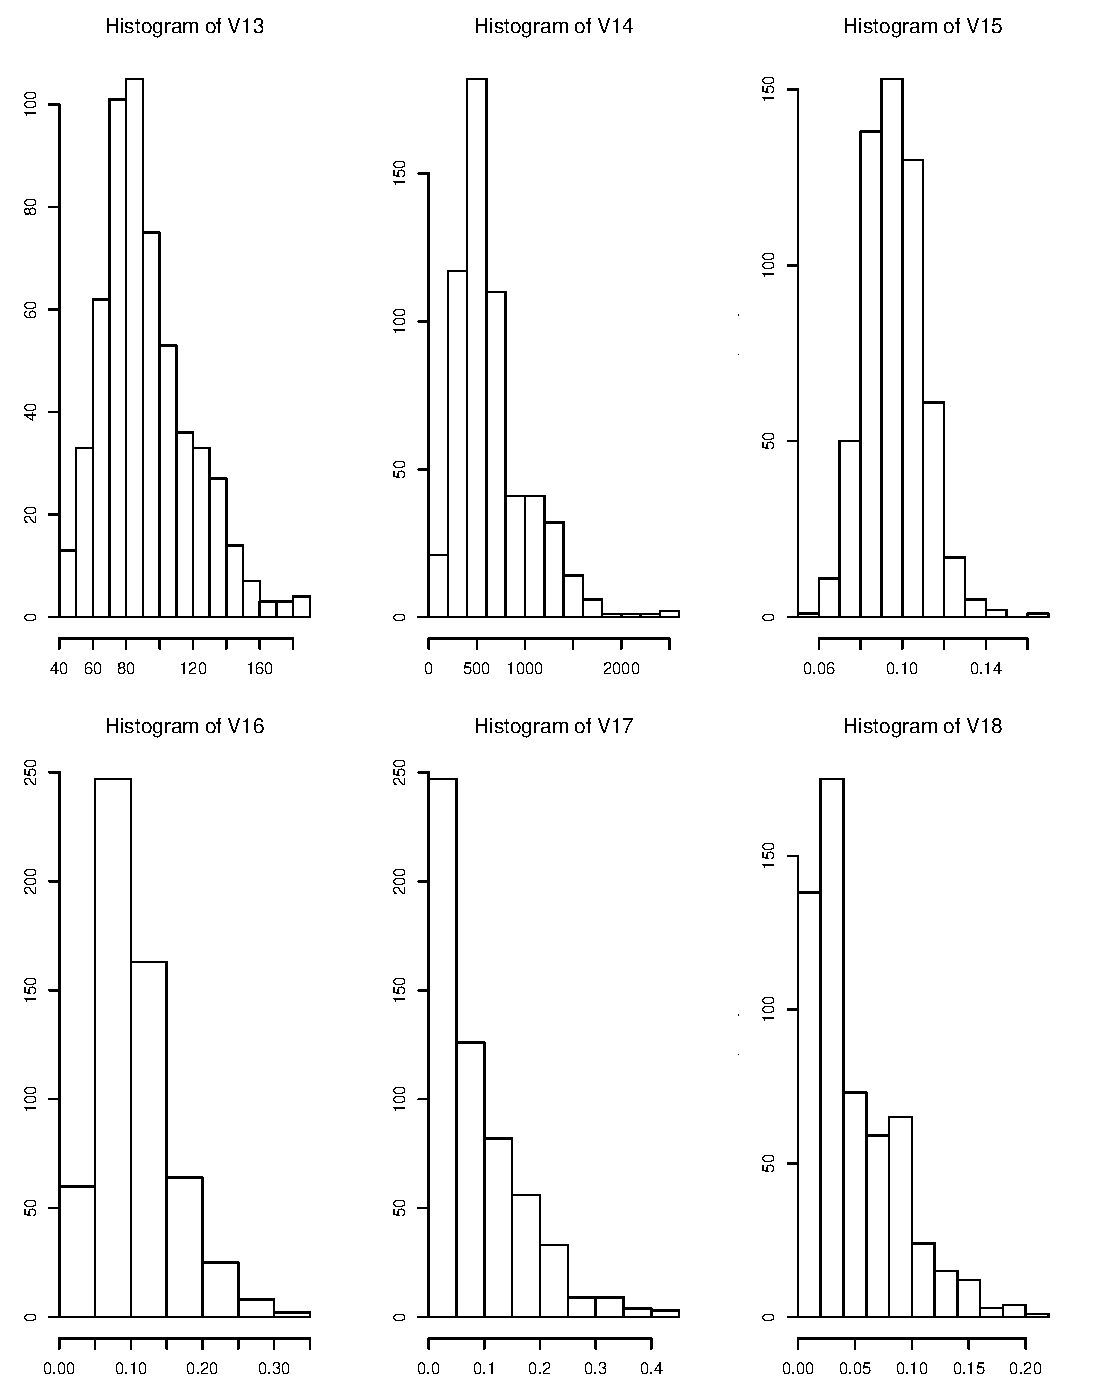
\includegraphics[scale=0.35]{histogram.pdf}
			\caption{Histogram of V13-V18}
			\label{fig:histogram}
		\end{subfigure}%
		\begin{subfigure}{.5\textwidth}
			\centering
			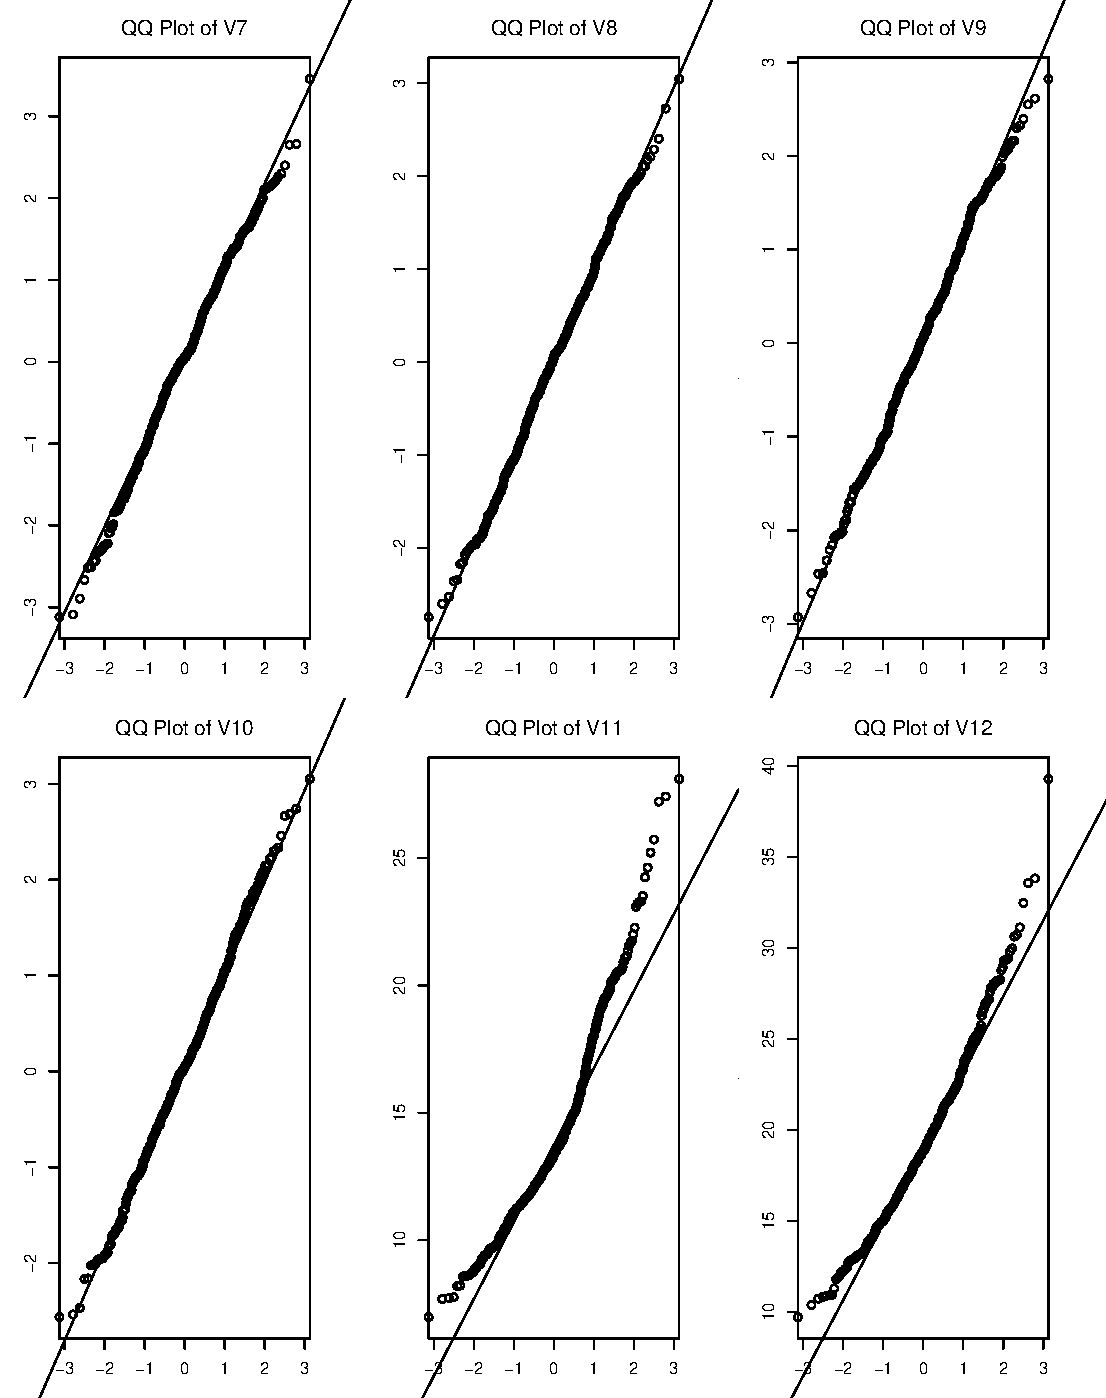
\includegraphics[scale=0.35]{qqplot.pdf}
			\caption{QQPlots of V7-V12}
			\label{fig:qqplot}
		\end{subfigure}
		\caption{Histograms and QQPlots}
		\label{fig: eda-1}
	\end{figure}
	
	
	
	\begin{figure}[H]
		\centering
		\begin{subfigure}{.5\textwidth}
			\centering
			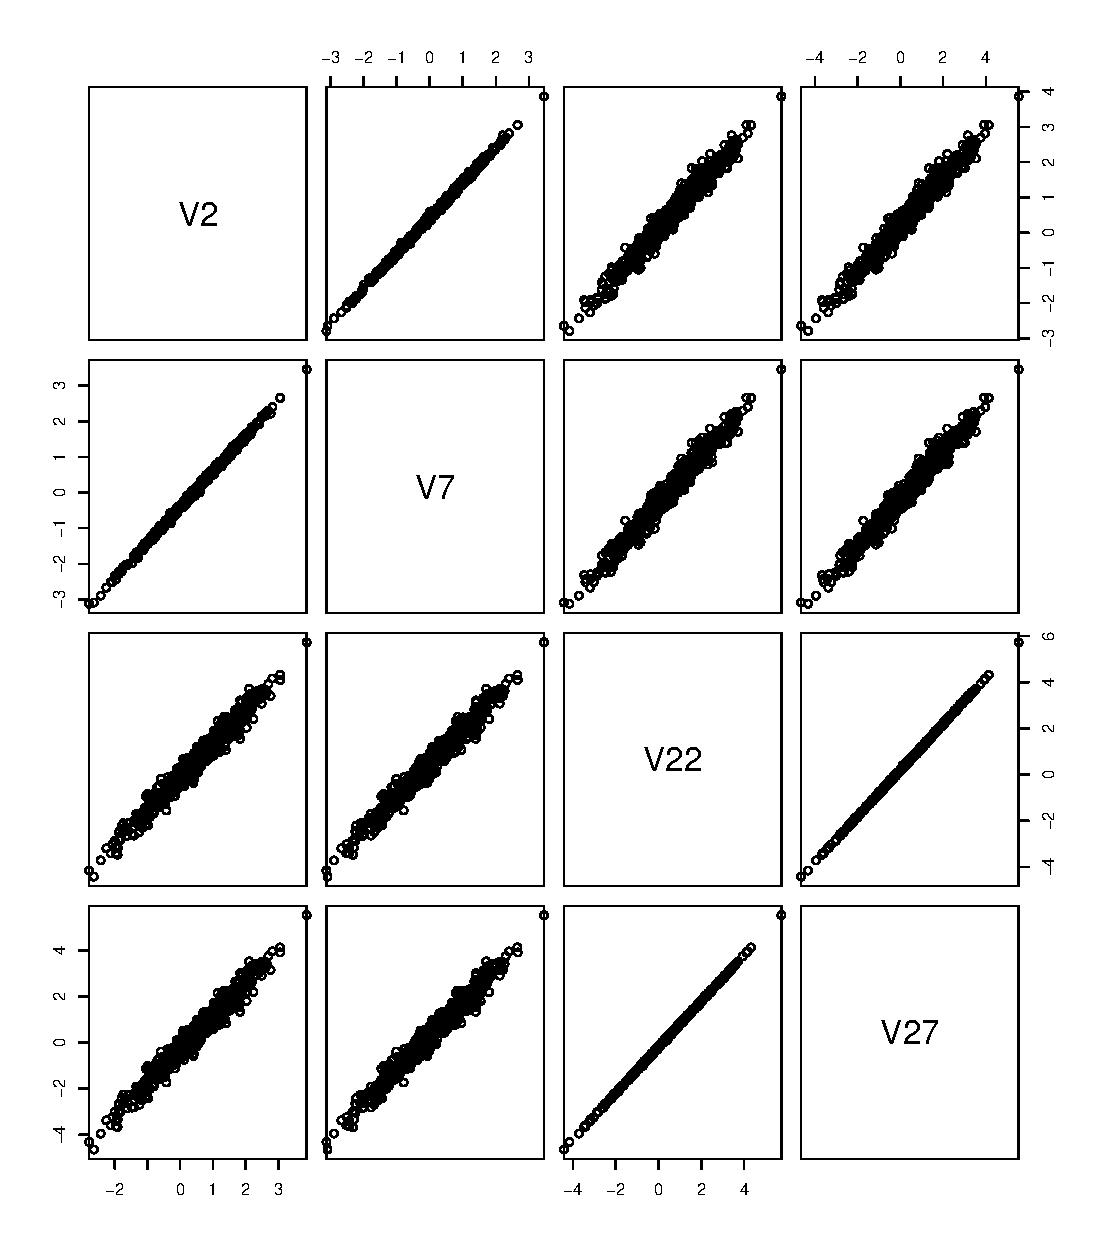
\includegraphics[scale=0.4]{pair.pdf}
			\caption{Scatterplot Matrices of (V2, V7, V22, V27)}
			\label{fig:pair}
		\end{subfigure}%
		\begin{subfigure}{.5\textwidth}
			\centering
			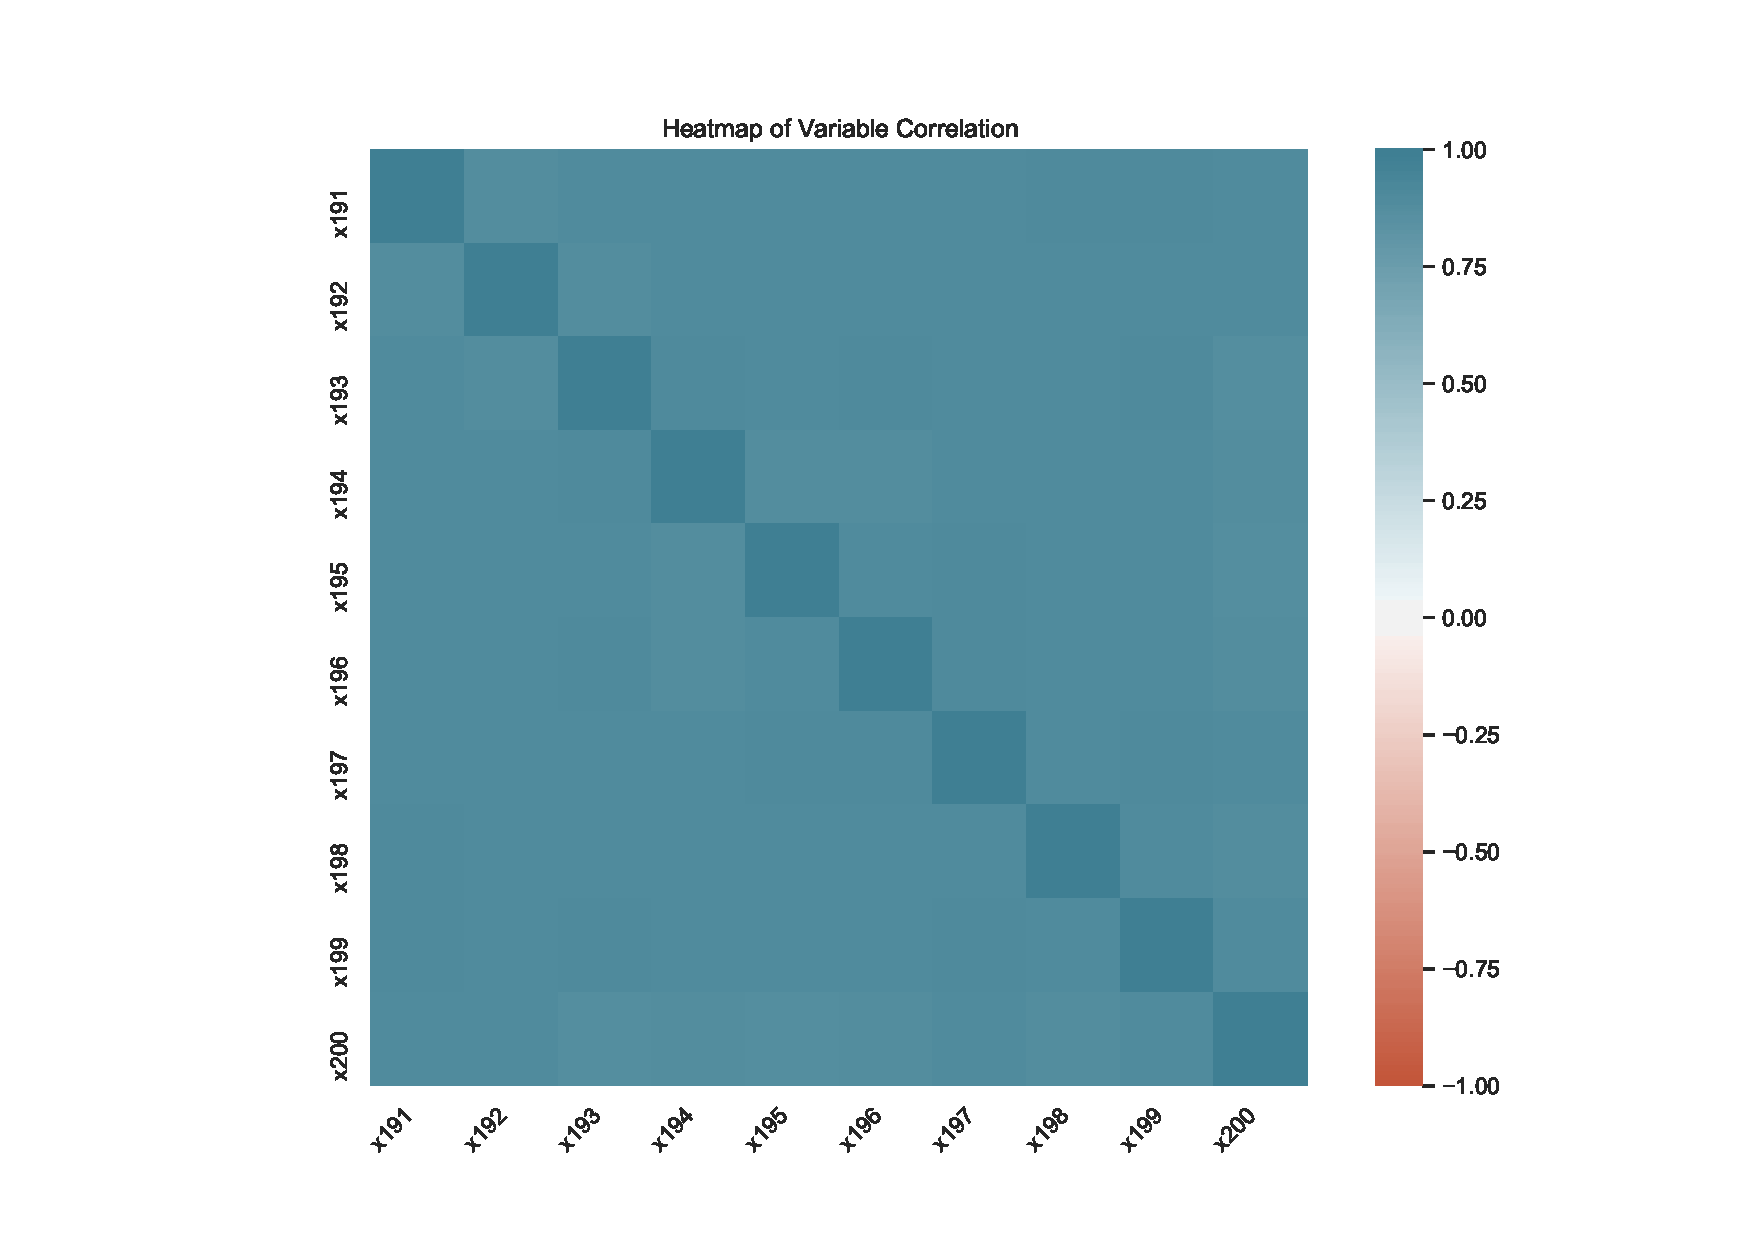
\includegraphics[scale=0.4]{heatmap.pdf}
			\caption{Heatmap of Correlations}
			\label{fig:heatmap}
		\end{subfigure}
		\caption{Scatterplot Matrices and Heatmap}
		\label{fig: eda-2}
	\end{figure}
	
	\begin{figure}[H]
		\centering
		\begin{subfigure}{.5\textwidth}
			\centering
			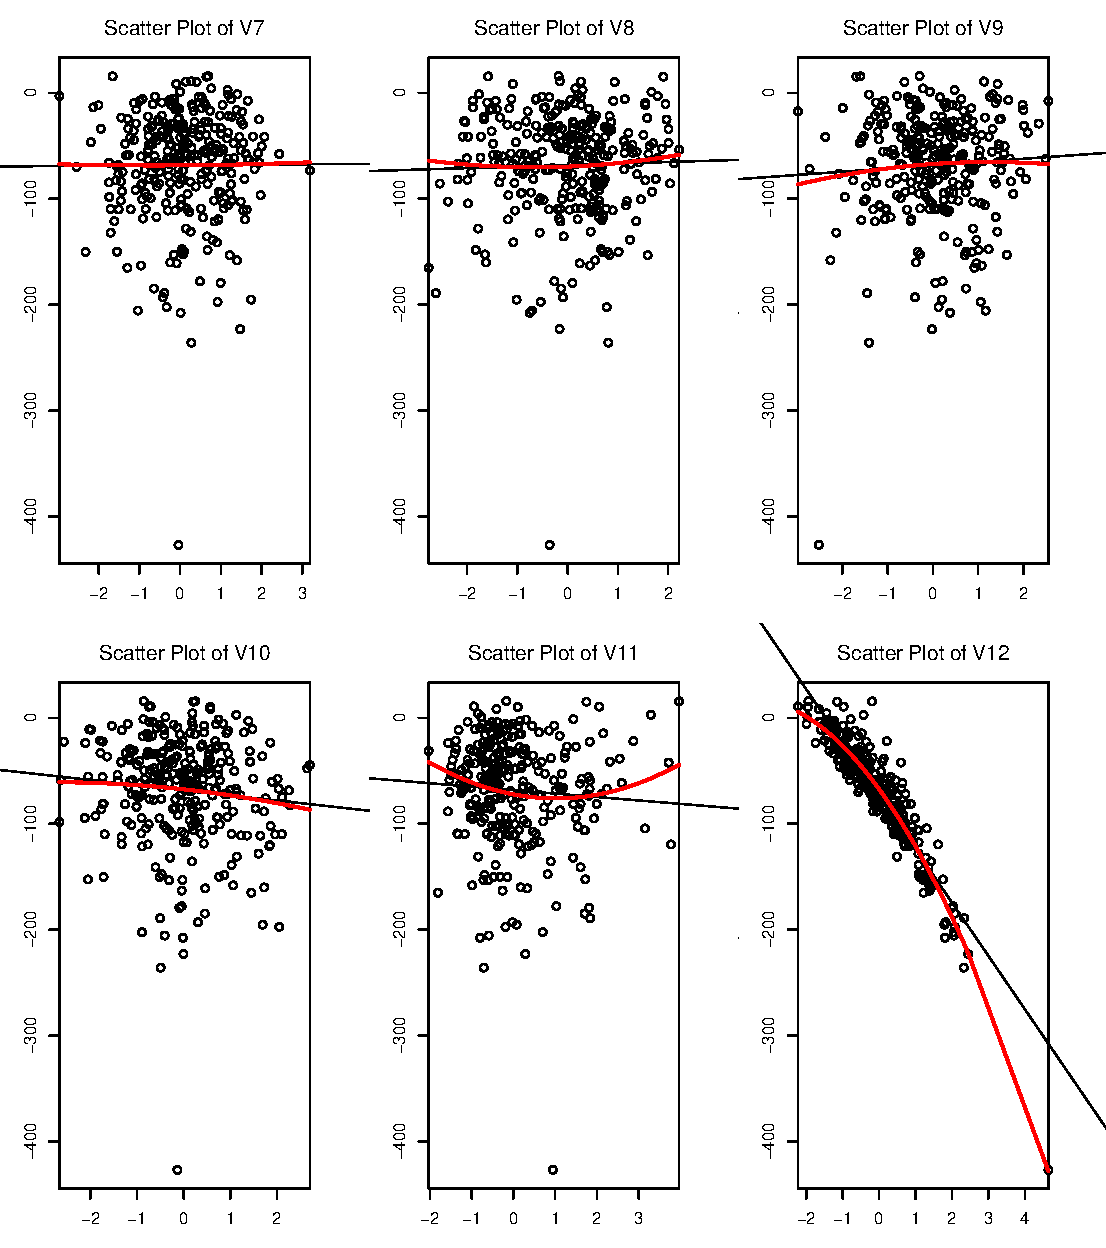
\includegraphics[scale=0.46]{scatterplot.pdf}
			\caption{Scatterplots of V7-V12 with linear and quadratic fit}
			\label{fig:scatterplot}
		\end{subfigure}%
		\begin{subfigure}{.5\textwidth}
			\centering
			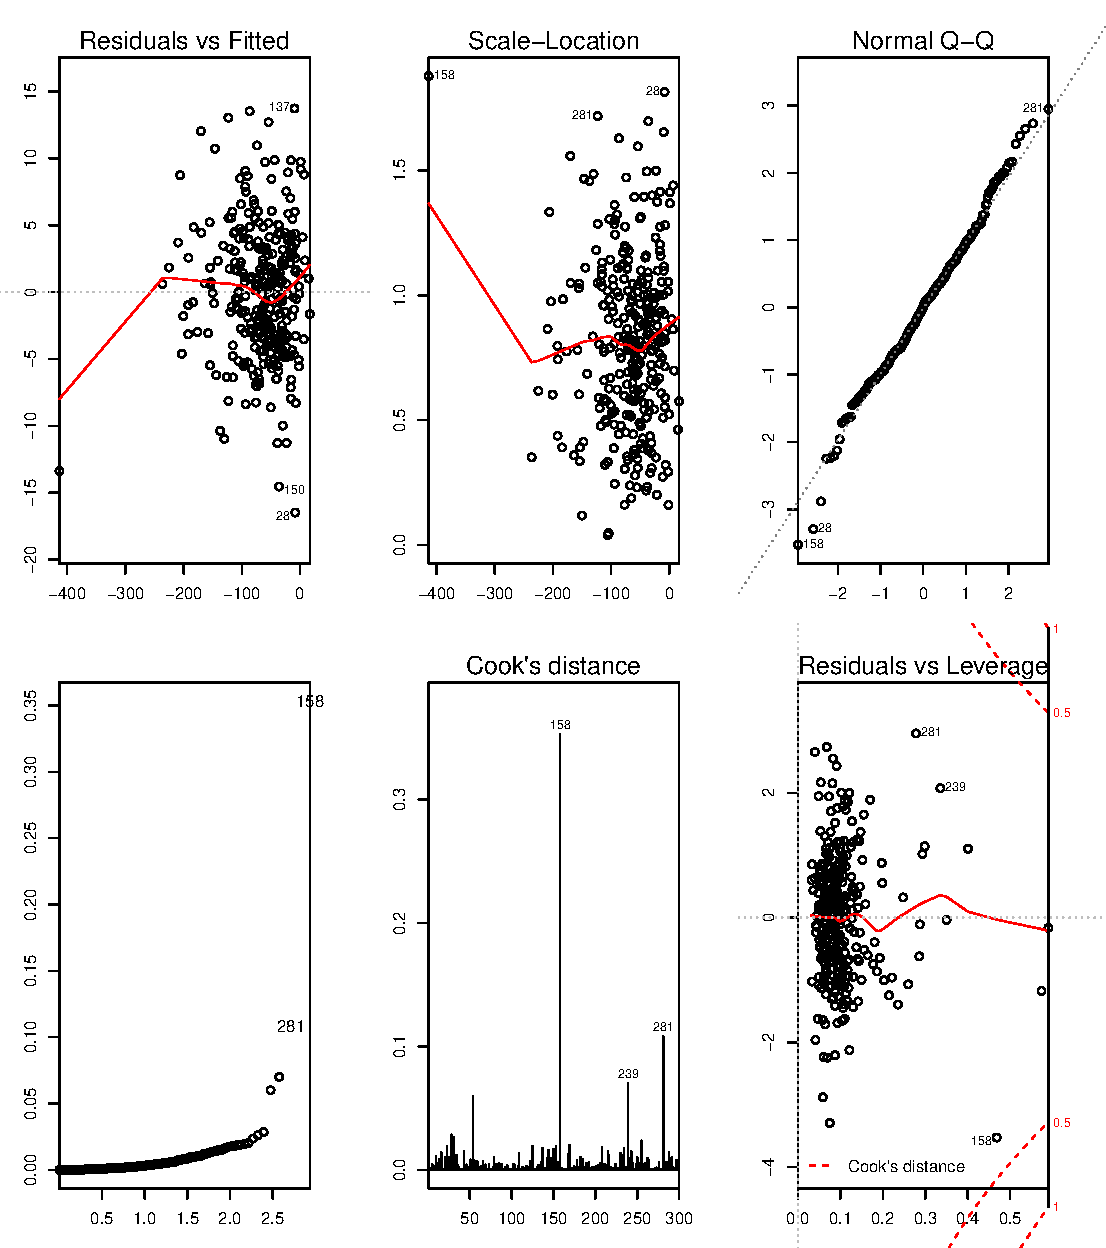
\includegraphics[scale=0.46]{diagnostic1.pdf}
			\caption{Residual Analysis}
			\label{fig:diagnostic-0}
		\end{subfigure}
		\caption{Scatterplots and Residual Analysis}
		\label{fig:eda-3}
	\end{figure}
	
	\begin{figure}[H]
		\centering
		\begin{subfigure}{.5\textwidth}
			\centering
			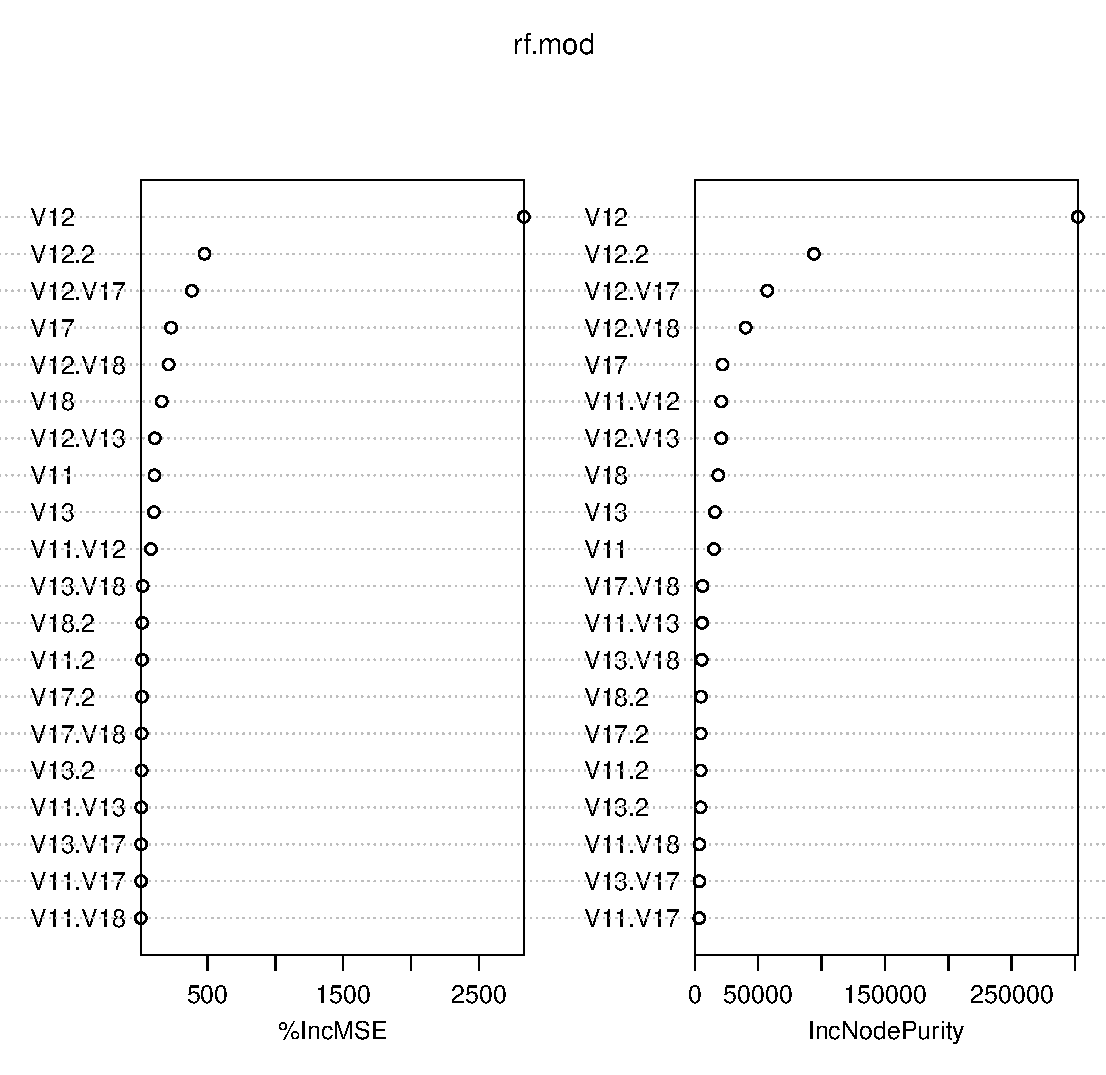
\includegraphics[scale=0.45]{2019Q2_comp9_rf_imp.pdf}
			\caption{Random Forest Feature Importance}
			\label{fig:rf_imp}
		\end{subfigure}%
		\begin{subfigure}{.5\textwidth}
			\centering
			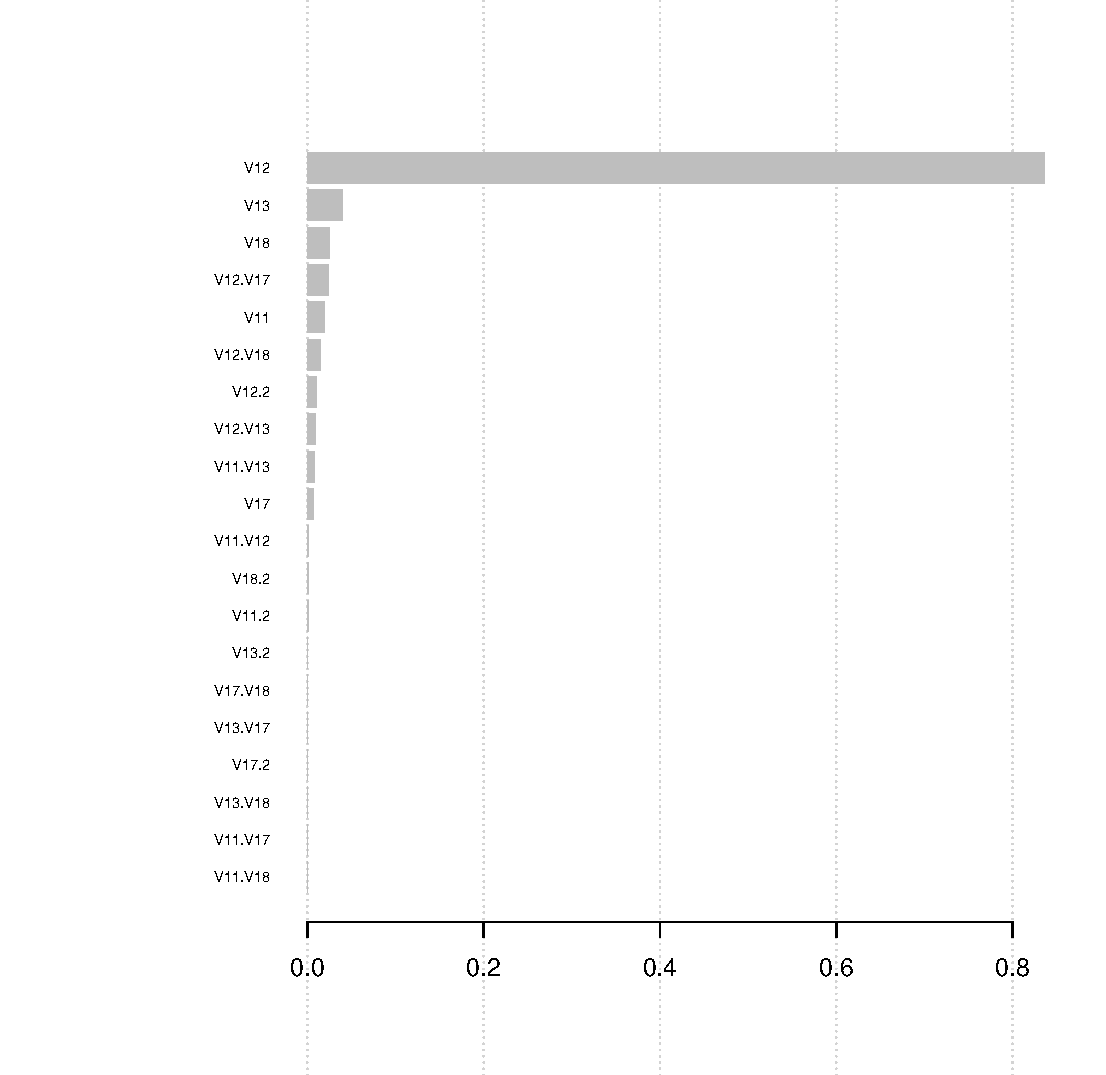
\includegraphics[scale=0.5]{2019Q2_comp9_xgb_imp.pdf}
			\caption{XGBoost Feature Importance}
			\label{fig:xgb_imp}
		\end{subfigure}
		\caption{Feature Importances of Comp 9}
		\label{fig:comp9_imp}
	\end{figure}
	
	
	
	\begin{figure}[H]
		\centering
		\begin{subfigure}{.5\textwidth}
			\centering
			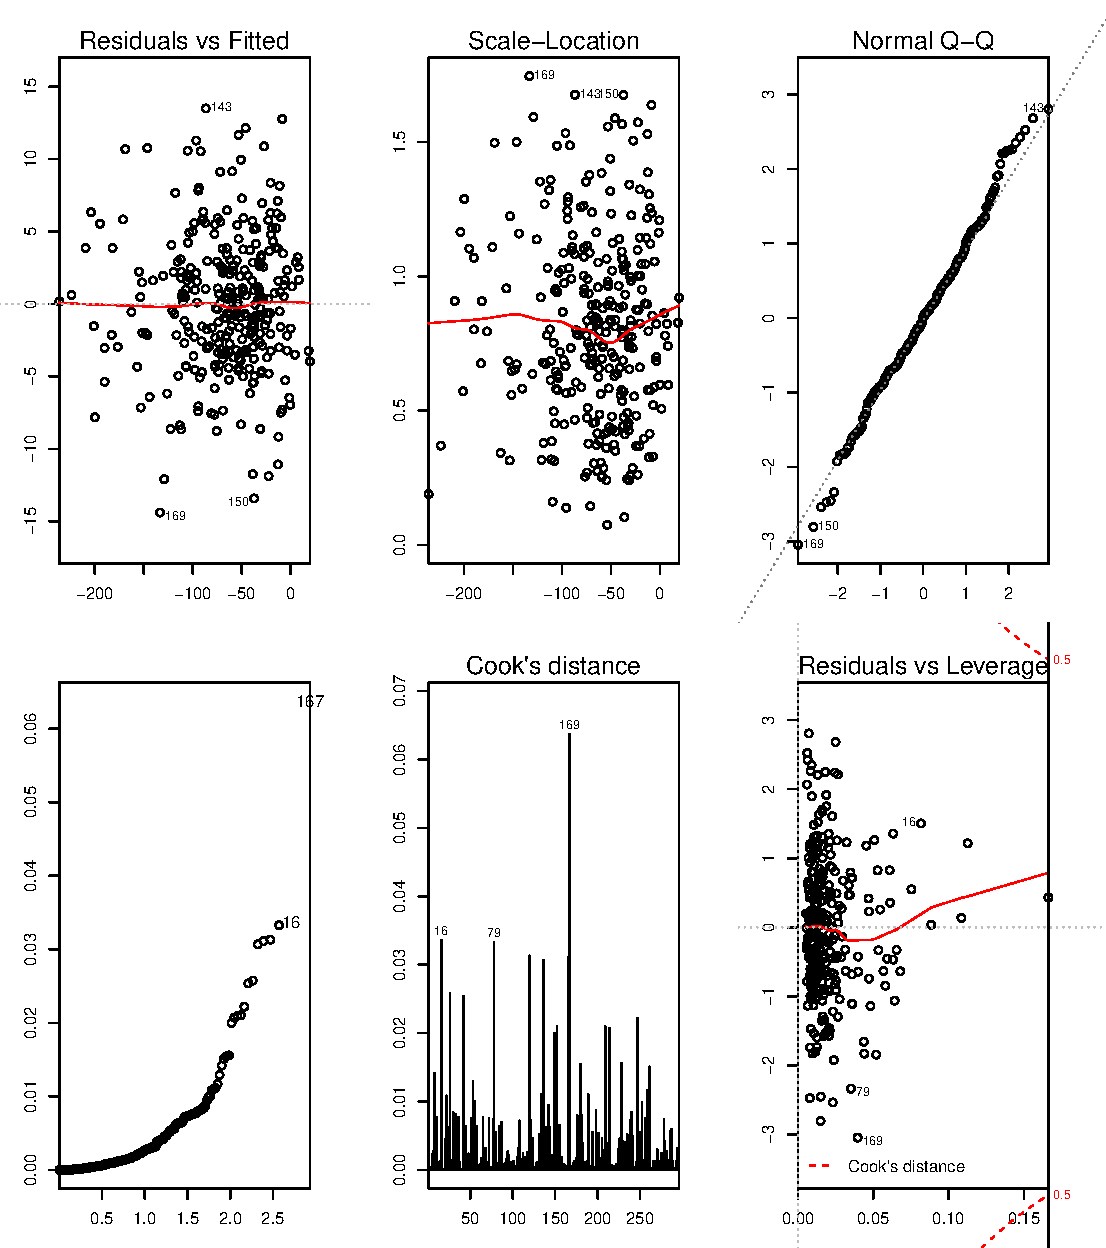
\includegraphics[scale=0.45]{diagnostic2.pdf}
			\caption{Random Forest Feature Importance}
			\label{fig:diagnostic-2}
		\end{subfigure}%
		\begin{subfigure}{.5\textwidth}
			\centering
			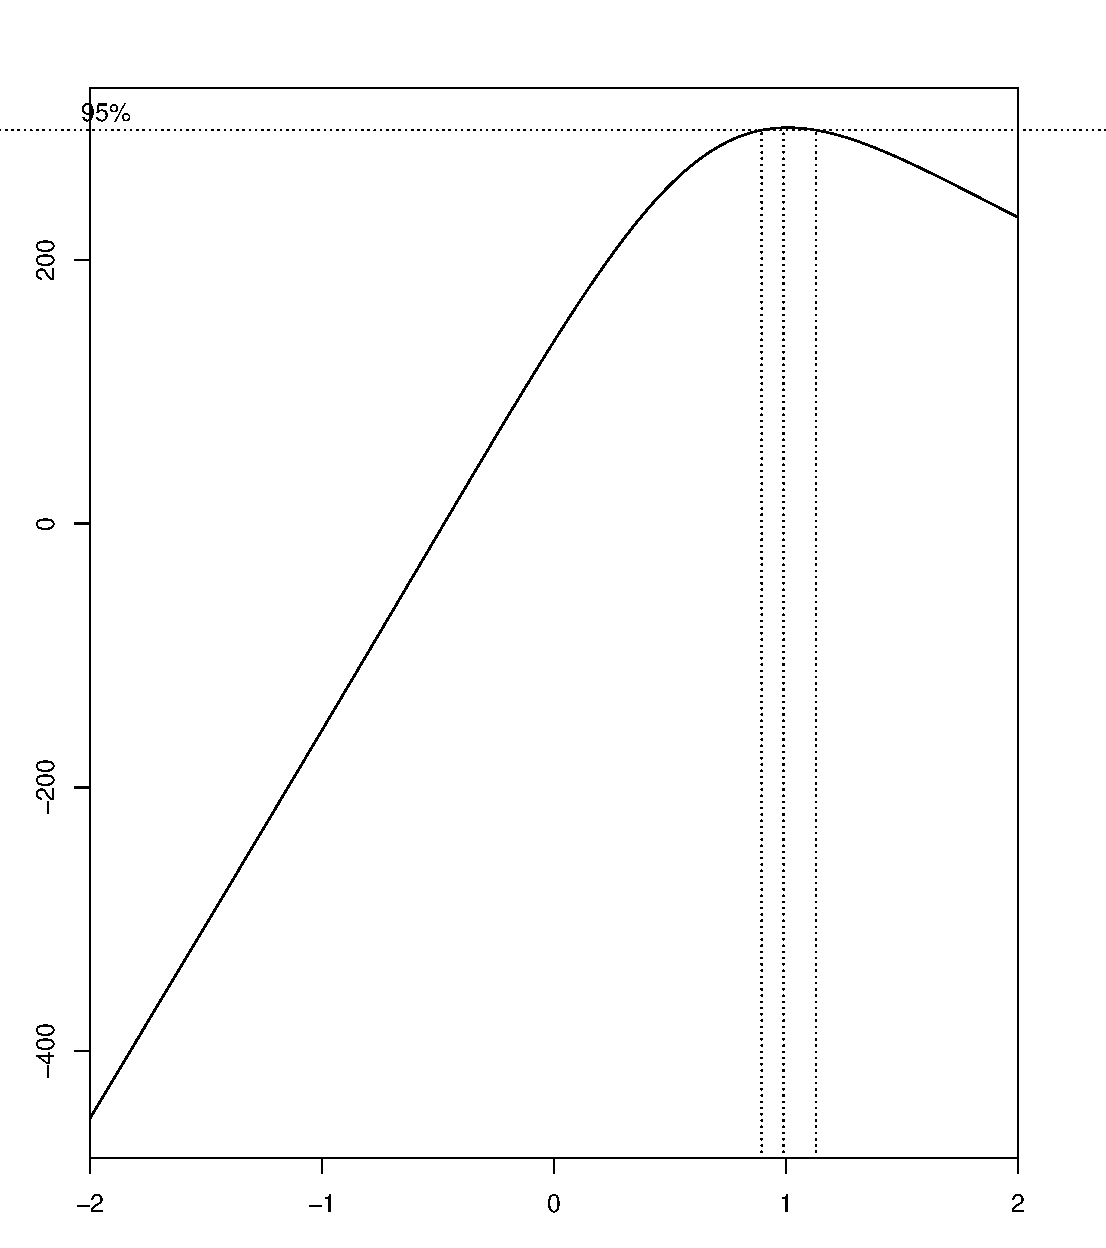
\includegraphics[scale=0.45]{boxcox.pdf}
			\caption{XGBoost Feature Importance}
			\label{fig:boxcox}
		\end{subfigure}
		\caption{Feature Importances of Comp 9}
		\label{fig:Final Model Diagnostics}
	\end{figure}
	
	
	
	\subsection*{Appendix B: Tables}
	
	
	\begin{table}[H]
		\centering
		\caption{Model Comparison Results}
		\begin{tabular}{|l|r|r|r|r|r|r|r|r|r|r|r|}
			\hline
			metrics   & Comp1  & Comp2   & Comp3  & Comp4  & Comp5  & Comp6  & Comp7  & Comp8  & Comp9  & Comp10 & Comp11 \\ \hline
			aic.err   & 27.22  & 0.00    & 25.02  & 41.81  & 41.81  & 28.75  & 27.80  & 27.08  & 25.53  & 25.01  & 25.42  \\ \hline
			aic.sd    & 6.21   & 0.00    & 5.49   & 14.33  & 14.33  & 5.97   & 5.82   & 6.23   & 5.40   & 5.39   & 5.05   \\ \hline
			bic.err   & 24.99  & 0.00    & 25.04  & 28.98  & 28.98  & 26.59  & 26.10  & 25.91  & 25.58  & 25.24  & 25.60  \\ \hline
			bic.sd    & 5.18   & 0.00    & 5.50   & 7.02   & 7.02   & 5.62   & 5.64   & 5.62   & 5.74   & 5.61   & 5.54   \\ \hline
			ridge.err & 94.15  & 1909.24 & 92.67  & 72.71  & 72.71  & 61.74  & 60.55  & 56.30  & 54.13  & 53.21  & 52.85  \\ \hline
			ridge.sd  & 28.22  & 401.99  & 33.86  & 21.17  & 21.17  & 17.76  & 17.52  & 16.24  & 15.33  & 14.60  & 13.90  \\ \hline
			lasso.err & 66.34  & 26.97   & 67.70  & 26.11  & 26.11  & 25.44  & 25.57  & 25.39  & 25.00  & 25.04  & 25.34  \\ \hline
			lasso.sd  & 18.83  & 6.69    & 19.43  & 6.03   & 6.03   & 5.63   & 5.63   & 5.56   & 5.60   & 5.72   & 5.66   \\ \hline
			mcp.err   & 67.22  & 27.06   & 69.43  & 26.76  & 26.76  & 27.00  & 26.98  & 26.44  & 25.59  & 25.67  & 25.68  \\ \hline
			mcp.sd    & 19.51  & 6.26    & 19.09  & 5.50   & 5.50   & 5.48   & 5.59   & 5.58   & 5.42   & 5.34   & 5.32   \\ \hline
			scad.err  & 67.77  & 28.21   & 68.38  & 26.81  & 26.81  & 26.50  & 26.49  & 26.13  & 25.52  & 25.41  & 25.79  \\ \hline
			scad.sd   & 19.70  & 6.62    & 19.54  & 5.65   & 5.65   & 5.63   & 5.71   & 6.14   & 5.51   & 5.57   & 5.54   \\ \hline
			xgb.err   & 56.99  & 82.21   & 57.80  & 69.96  & 67.49  & 67.58  & 66.93  & 68.93  & 61.17  & 63.65  & 63.45  \\ \hline
			xgb.sd    & 17.02  & 39.34   & 20.57  & 27.20  & 31.27  & 31.17  & 26.46  & 34.55  & 24.78  & 27.36  & 29.08  \\ \hline
			rf.err    & 311.80 & 305.62  & 269.86 & 254.14 & 246.97 & 248.41 & 240.44 & 208.60 & 210.42 & 218.13 & 214.36 \\ \hline
			rf.sd     & 131.43 & 157.61  & 145.40 & 120.39 & 128.22 & 130.66 & 125.87 & 105.34 & 108.53 & 119.28 & 107.37 \\ \hline
		\end{tabular}
		\label{table:model_comparison}
	\end{table}
	
	
	
	\begin{table}[H]
		\centering
		\caption{Comparison - Subset Correspondence}
		\begin{tabular}{|l|l|}
			\hline
			comp1                                                  & comp2                                                              \\ \hline
			(V1-V30)                                               & (V1-V30)\textasciicircum{}2                                        \\ \hline
			comp3                                                  & comp4                                                              \\ \hline
			(V4, 8, 11, 12, 13, 14, 17, 18, 20, 22, 27, 28)        & (V4, 8, 11, 12, 13, 14, 17, 18, 20, 22, 27, 28)\textasciicircum{}2 \\ \hline
			comp5                                                  & comp6                                                              \\ \hline
			(V4, 8, 11, 12, 13, 17, 18, 20, 28)\textasciicircum{}2 & (V8, 11, 12, 13, 17, 18, 20, 28)\textasciicircum{}2                \\ \hline
			comp7                                                  & comp8                                                              \\ \hline
			(V11, 12, 13, 17, 18, 20, 28)\textasciicircum{}2       & (V11, 12, 13, 17, 18, 20)\textasciicircum{}2                       \\ \hline
			comp9                                                  & comp10                                                             \\ \hline
			(V11, 12, 13, 17, 18)\textasciicircum{}2               & (V11, 12, 13, 17)\textasciicircum{}2                               \\ \hline
			comp11                                                 &                                                                    \\ \hline
			(V11, 12, 13, 18)\textasciicircum{}2                   &                                                                    \\ \hline
		\end{tabular}
		\label{tab: comp-subset}
	\end{table}
	
	
	
	
	\begin{table}[H]
		\centering
		\caption{Linear Model Comparison}
		\begin{tabular}{|l|l|l|}
			\hline
			model                                           & lm.err    & lm.sd    \\ \hline
			y $\sim$V11 + V12 + V13 + V17 + V12.2           & 23.655433 & 4.319979 \\ \hline
			y $\sim$V11 + V12 + V13 + V17 + V12.2 + V12.V17 & 24.650799 & 5.522014 \\ \hline
			y $\sim$V11 + V12 + V13 + V18 + V12.2 + V12.V18 & 24.728938 & 5.373833 \\ \hline
			y $\sim$V11 + V12 + V13 + V18 + V12.2           & 24.71344  & 5.32118  \\ \hline
		\end{tabular}
		\label{table:lm_comp}
	\end{table}
	
	
	
	
	\begin{table}[H]
		\centering
		\caption{Reliability Measure of Feature Selection}
		\begin{tabular}{|c|c|c|c|c|}
			\hline
			VSD & VSD- & VSD+ & F-measure & G-measure\\
			\hline
			16.00856 & 1 & 15.00856 & 0.3332239 & 0.4103058 \\
			\hline
		\end{tabular}
		\label{tab:reliability_measure}
	\end{table}
	
	
	\begin{table}[H]
		\centering
		\caption{Linear vs. Nonparametric Comparison}
		\begin{tabular}{|l|l|l|}
			\hline
			model                                 & err   & sd     \\ \hline
			y $\sim$V11 + V12 + V13 + V17 + V12.2 & 23.79 & 4.36   \\ \hline
			XGBoost                               & 56.99 & 17.02  \\ \hline
			Random Forest                         & 311.8 & 131.43 \\ \hline
		\end{tabular}
		\label{table:lm_nonparam_comp}
	\end{table}
	
	
	\subsection*{Appendix C: Text Results}
	\noindent\textbf{Result 1: Features selected in Comp 1}
	\verbatiminput{Results/comp1.txt}
	
	\noindent\textbf{Result 2}
	
	\verbatiminput{Results/comp2.txt}
	
	
	\noindent\textbf{Result 3}
	
	\verbatiminput{Results/comp9.txt}
	
	\noindent\textbf{Result 4}
	
	\verbatiminput{Results/mod-summary.txt}
	
	
%\end{document}